\section{Vurdering}
På bagrund af graferne i sektion \ref{ch4_design} kan det konkluderes, at det designede FIR-filter formår at filtrere frekvensen $\omega_2=\frac{\pi}{2}$ fra det samplede signal $s[n]$ som ønsket ved anvendelse af orden større end $30$. \\
Figur \ref{fig:filter_rekt} illustrerer, at de opstillede specifikationer til en vis grad overholdes ved en orden på hhv. 30 og 100 og anvendelse af det rektangulære vindue. Det ses tydeligt, at transitionsbåndet bliver smallere jo højere orden der anvendes. De ripples, der forekommer i pasbåndet formindskes også, når ordenen øges. Dog forsvinder de ikke, da det er det rektangulære vindue, der anvendes. Som nævnt kan dette optimeres ved at ændre på vinduet. Herunder optimeres filteret.

\section{Optimering}
Ud fra ovenstående forsøges der med højere filterorden. Således opnås der en god filtrering ved $M=92$ således frekvensen $\pi/2$ filtreres fra uden de andre frekvenser påvirkes meget. Dette resultat ses på figur \ref{fig:resultat}.
\begin{figure}[H]
\begin{minipage}{0.49\textwidth}
\centering
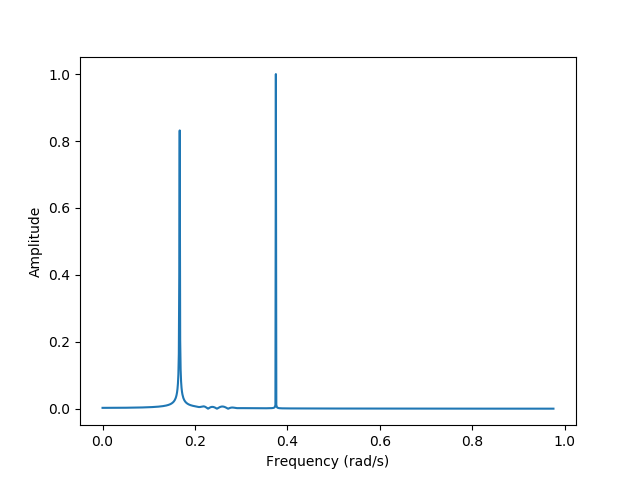
\includegraphics[width=\textwidth]{figures/sf1.png}
\caption{Amplituderespons for filter af orden $M=92$.}
\end{minipage}
\begin{minipage}{0.49\textwidth}
\centering
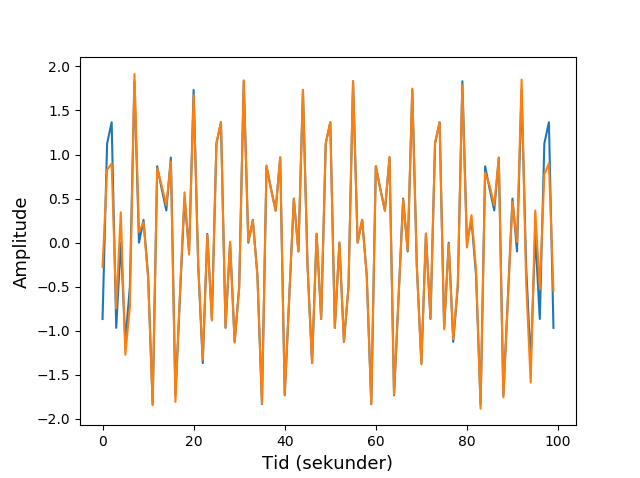
\includegraphics[width=\textwidth]{figures/sf.png}
\caption{Ideelle signal filtrerede signal (blå) med det filtrerede signal (orange).}
\end{minipage}
\end{figure}
Amplituderesponsen for Hammingvinduet brugt til filteret ses desuden på figur \ref{fig:amplituderespons} i bilag \ref{app2}.






